\chapter{E2E-VIV Explained\ifdraft{ (Philip/Daniel/Adam) (100\%)}{}}
\label{chapter:e2e_viv_explained}

\section{Election Process and Goals}
\begin{wrapfigure}{l}{1.6in}
\vspace*{-4ex}
\begin{center}
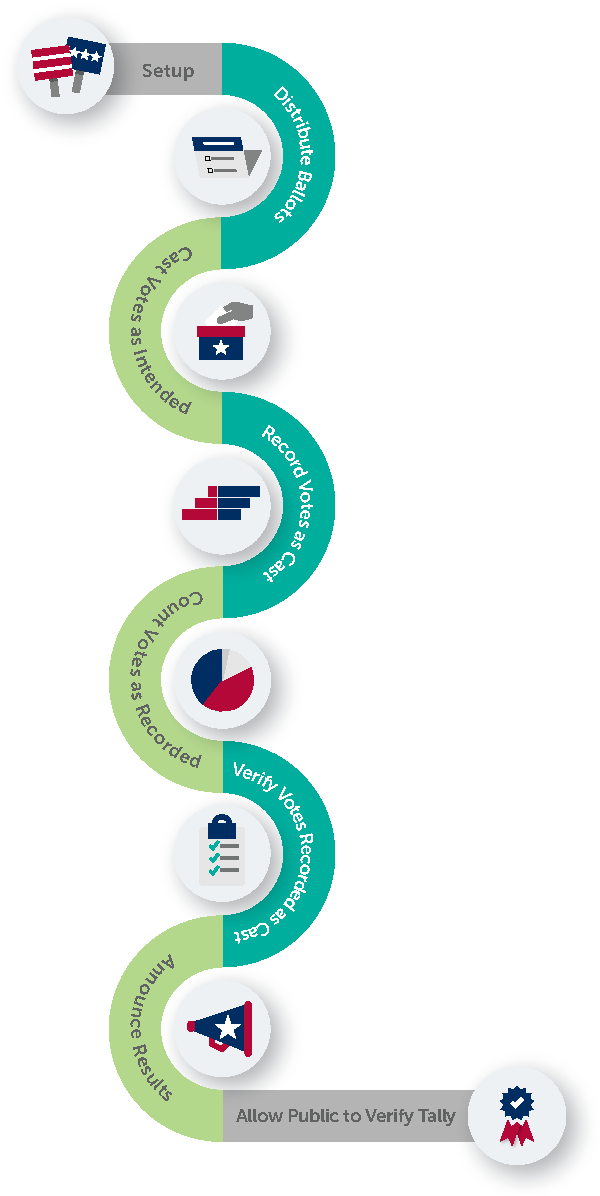
\includegraphics[width=2.8in]{e2e_viv_explained_resources/process.pdf}
\end{center}
\label{fig:e2eviv_process_illustrated}
\end{wrapfigure}
A typical Internet voting election process has six phases:

\begin{description}
  \item[\textbf{SETUP.}] During the setup phase, election officials gather 
    information needed to run the election. This includes:
    \begin{itemize}
     \item gathering registration information for all voters;
     \item identifying the issues and races that will be voted on;
     \item designing ballots, often in multiple languages, for all
       precincts participating in the election;
     \item sending instructions and other information about the
       election to voters; and so on.
    \end{itemize}
  \item[\textbf{DISTRIBUTION.}] Different voting systems use different
    mechanisms to distribute ballots to voters, such as postal mail,
    email, or a website that provides downloadable ballots.
  \item[\textbf{VOTING.}] Voters fill out their ballots, often with the help of
    software installed on their own computers.
  \item[\textbf{CASTING.}] Election officials receive the completed ballots. As
    with distribution, different voting systems use different ballot
    casting mechanisms.
  \item[\textbf{TALLYING.}] The tallying phase includes the remainder of the
    tasks that finalize the election. Counting votes and announcing
    the election outcome are common to almost every election system,
    though some include other tasks such as publishing information
    needed for audits.
  \item[\textbf{AUDITING.}] Some elections will inevitably be disputed. In such
    cases, there is a final phase in which interested parties look for
    evidence that the election outcome is correct (or incorrect).
\end{description}

\clearpage\break

One major concern for Internet voting involves ballot integrity during the
distribution, voting, and casting phases. For the election outcome to be
correct, it is important that:
\begin{itemize}
\item the blank ballot that is received by and displayed to the voter
  match the ballot created and sent by the election officials;
\item the computer used to fill out the ballot faithfully reports the
  intention of the voter; and
\item the filled out ballot received by the election officials is the
  same as it was when the voter sent it.
\end{itemize}
Typical Internet communications involve not just the computers owned
by the two parties communicating, but also many intermediary computers
controlled by neither party. For example, an email you send from
anywhere in the world will travel through multiple servers on its way
to its destination. At any point, one of these servers could intercept
and modify the email without your knowledge. A good election system
needs to account for this, making it impossible for these
intermediaries to intercept ballots for viewing or modification during
transit.

Another concern is that most voters are not system administration
experts, and many of their computers are compromised by malware. A
compromised computer may corrupt the voting phase: even if the voter
receives an unaltered ballot, malware may change the way the ballot is
displayed or the way the vote is recorded before casting the
ballot. It can be difficult to design a system that can resist this
kind of attack without significantly reducing the usability of the
system. Some systems, referred to as dual (or triple) channel systems,
use alternative distribution mechanisms as cross-checks. For example,
election officials may send a code by postal mail that a voter can use
to check that a displayed ballot is correct.

As much as possible, Internet voting should be private and
anonymous. It is essential that voters are free to vote the way they
choose, and do not feel pressured to vote for a particular candidate
or vote a particular way on any issue. The fewer people who know or
can find out how a voter voted, the more comfortable the voter can
feel about privacy.

At the same time, election systems must only record votes from people
who are registered to vote, and must only record one vote from each
voter. Election systems must balance the need to keep votes anonymous
agsinst the need to ensure that a vote is coming from somebody who
should to be able to vote.
% I keep struggling with the fact that I think vote and ballot are two different things and that you are using them 
% interchangeably. A ballot can have many votes on it... I think people cast "ballots". 
% Is it "vote casting" or as I would say it ballot casting - they vote by casting a ballot,
% election officials record one ballot to a voter, but that ballot could contain
% many votes on it... isn't the ballot tied to the voter, and then the votes to the ballot,
% or maybe, I am using this language wrong - just thought I would note it. 
%\tododmwit{ask Joe for a reference to the audit that showed that voting
%terminal logs retained exactly who voted for what}

One popular approach to this problem in existing systems is to require
that each vote be tied to the voter who cast it long enough to decide
whether to include the vote in the later tally or not. After it is
decided to include the vote, the system records the vote and deletes
the information about who cast it. This approach can work; however,
audits of systems that take this approach have shown that it is easy
to accidentally retain the connection between votes and voters longer
than intended. This makes information much more widely visible than
intended. It would be better if voters could be confident that the
system does not store any connections between their votes and their
identities. To accomplish this, the information a voter returns during
the ballot casting phase must not include any personally identifying
material.

This is a subtle, but crucial, distinction. The overall objective is
for Internet voting systems to be correct, private, secure, and so
forth. It is important for the people who develop these systems to
verify that they are correct and take an active role in seeking out
and eliminating defects in the system. However, verifiable Internet
voting goes even farther: the system must be \emph{visibly}
correct. That is, voters using the system must be able to \emph{check}
that it is behaving correctly, without trusting that the system has no
bugs or trusting that the system's behavior has not been influenced by
third parties. It is especially difficult to prove to voters that
their personal information has been deleted in order to protect their
privacy, so voters may not want to provide their information in the
first place.

This is why it is critical that an Internet voting system not only be
correct, but \emph{verifiably} correct. Verifiability is one of the
central concerns of Internet voting, and is a critical part of the
defense against the software bugs, security vulnerabilities, and
sophisticated cybercrimes that history tells us are sure to occur.

The tallying process provides a particularly good example of the
difference between correctness and verifiability. Voters certainly
want the election system to count the votes correctly, but the goal of
verifiability is to provide some \emph{evidence} to voters that the
election outcome is correct. Different systems attempt this in
different ways. For example, they may allow voters to check that:

\begin{itemize}
\item their vote was included in the election outcome; 
\item the system is recording the content of their
votes correctly; or
\item the number of people that voted for a given candidate is
  accurately calculated (this must be proven without revealing any of
  the individual votes).
\end{itemize}

Meeting these verification objectives without violating anonymity and
privacy is a balancing act. Each of these individual objectives
contribute to a single top-level goal: \emph{end-to-end verifiability}.
``End-to-end'' means that the whole election process produces a result
that matches the intentions of the voters.

The verification objectives can be summarized with the catchphrase,
``Cast as intended; recorded as cast; and counted as recorded.''

\begin{itemize}
\item ``Cast as intended'' is the demand that casting use secure
  communications and other mechanisms to ensure that malware and
  outsiders cannot change the vote.
\item``Recorded as cast'' is the demand that the election system
  itself correctly interprets a vote.
\item ``Counted as recorded'' is the demand that the tallying process
  be accurate.
\end{itemize}

These demands are subject not only to correctness but also to
verifiability, so that voters can believe these properties hold even
if they suspect that the systems, or the election officials, are
corrupt.

\section{Shortcomings and Expectations of E2E-VIV}

As discussed in \autoref{chapter:remote_voting}, several difficulties
exist with current voting processes:

\begin{itemize}
\item voters with disabilities cannot vote unassisted; 
\item communication channels with remote voters are often slow and
  unreliable;
\item vote tallying is labor-intensive and error-prone; 
\item election audits are costly; and
\item there is little visibility into the election process, so voters
  (and, in some cases, even auditors) must trust the reports of
  election officials and voting hardware vendors on election outcomes
  and processes.
\end{itemize}

Internet voting may be able to alleviate some of these
concerns. Voters with disabilities could potentially use their own
familiar hardware, such as Braille displays, screen readers,
sip-and-puff input devices, and others, to participate in the
election. Internet communications are traditionally speedy (taking
seconds rather than weeks) and relatively robust compared to overseas
postal mail. In most systems, tallying is automated and fast. Auditing
can still be a challenge, though it is expected that verifiable
systems can make elections more transparent for this purpose. However,
implementation of Internet voting has its own challenges. A system
that properly addresses privacy and security concerns may be too
complex to use and maintain or too costly to deploy.

\section{E2E-VIV in Practice}

Several practical voting systems have been developed based on the
principles of E2E-VIV. This section describes some systems that
communities have used in real elections or pilot tests.

\subsection{RIES}
\label{sec:ries} 

RIES, the Rijnland Internet Election System~\cite{hubbers2004}, was
first used in 2004 to support elections to the Rijnland water
management board. RIES supplemented the system of postal voting
already in use. Election officials used a later version of RIES to
allow expatriate voters to participate in the Dutch parliamentary
elections~\cite{gonggrijp2009}.

Before a RIES election, credentials---in the form of a very long
number---and instructions are sent by postal mail to every voter.

During the election, each voter logs into the election website. The
website includes a voting application written in JavaScript; the
voting application is a ``client-side'' application, which means that
it runs on the voter's computer and not on the election server. The
client-side application processes the voter's authorization code and
the public ID of the candidate to create an encrypted
vote. The encrypted vote is then placed on a public online ``bulletin
board'' that serves as a ballot box.

At the close of the polls, the election authority releases the final
vote tallies along with a codebook containing the encryptions of all
valid credentials and all candidate IDs.

The algorithms and protocols used by RIES are public, and each voter
has access to all of the inputs and outputs. In principle, each voter
may check the computations. This level of verifiability is weaker than
the desired individual verifiability of E2E-VIV, but is nonetheless
far stronger than conventional voting systems.

In 2006, the Organization for Security and Co-operation in Europe
(OSCE) sent an election assessment team to observe the use of
RIES. Their report~\cite{osce2007} stated that they could not observe
many critical security features of the system, and therefore could not
be certain of their effectiveness. In 2008, the Eindhoven Institute
for the Protection of Systems and Information (EiPSI) revealed several
weaknesses in RIES~\cite{hubbers2008}:

\begin{itemize}
  \item the voter self-check procedure is quite complicated;
  \item the two-channel (mail and Internet) voting makes the system
    less transparent;
  \item too much power is given to the election administrator and the
    system's Internet host;
  \item issues arise when modifying the codebook due to a revoked
    ballot; and
  \item realistic ways to forge votes via cryptographic means (in
    particular, using hash collisions) exist.
\end{itemize}

One of the more important lessons learned through RIES is that when
voter authorizations are distributed far in advance of the election, a
mechanism must be provided that allows voters to obtain replacement
credentials and invalidate lost credentials. This mechanism adds
significant complexity to the system, and is a source of some of the
problems reported in the OSCE and EiPSI reports.

Another feature of RIES, which has significant tradeoffs, is the
ability to perform testing during the election: pre-invalidated test
ballots are deliberately added to the bulletin board in order to test
the network path from selected Internet clients to the server. While
such testing can, in principle, increase confidence in the election
integrity, in practice it opens the system to spoofing and denial of
service\footnote{A \emph{spoofing} attack deceives the target into
  believing that an Internet communication came from somewhere other
  than its actual source. A \emph{denial of service} (DoS) attack is
  an attempt to make an Internet server unavailable to its intended
  users.} attacks. Moreover, the RIES implementation is aware when it
is processing test ballots rather than real ballots, and all of the
test ballots are typically voted identically from the same
computer. This significantly limits the confidence provided by such
testing, at the expense of increased system vulnerability.

Because of these critical reports, election officials discontinued
plans to use RIES in the 2008 Dutch parliamentary elections, and the
Netherlands banned Internet voting.

\subsection{Prêt à Voter}
\label{sec:pret-voter}

In 2007, the University of Surrey in the U.K. attempted to
use the Prêt à Voter system~\cite{chaum2005, burton2012} in a student
election~\cite{bismark2007}. This attempt was stopped prematurely, due
to system malfunctions and an inability to open polling at all polling
stations on time. The failure illustrated many of the pitfalls of
adapting a research system to an actual election, such as a short
timetable, a lack of clear requirements, and the need for rigorous
implementation practices.

Prêt à Voter uses two-part paper ballots. Candidate names appear on
one part and voting targets---the areas that voters must mark to cast
their votes---appear with a ballot ID number or barcode on the other
part. Typically, the two parts are printed as a single sheet with a
perforation to divide the sheet after voting.

From the voter's perspective, the order of the candidate names on the
ballot is random. The voter makes a mark next to the candidate name
she chooses, separates the two parts of the ballot, and destroys the
part containing the candidate names. She may take a copy of the voted
part home for later verification.

For tabulation, a cryptographically secure mapping exists from the
ballot ID numbers to the apparently-random orderings of the
candidates. The system uses this mapping to decode the cast ballots
into readable ballots with candidate names, while removing the
associations between ballots and their ID numbers. The decoded ballots
are then posted to a public online bulletin board.

Unvoted ballots may be audited before, during and after the election
to ensure that the decoding of cast ballots is being correctly
performed. Randomly selected stages in the decoding can be challenged
to prove the integrity of the count, and any interested party can
easily count the decoded ballots for verification.

Individuals may also search for their voted ballot IDs on the bulletin
board. This reveals the positions that were marked on that ballot but,
crucially, does not show the corresponding candidate names. A voter
can verify that the positions she marked at the polling place were
correctly recorded by the system, but because she no longer has the
part of the ballot linking candidate names to ballot positions, she
cannot prove to anyone else how she voted.

\subsection{Punchscan}
\label{sec:punchscan}

Punchscan~\cite{popoveniuc2006,popoveniuc2010punchscan} was used for
the graduate student association elections of the University of Ottawa
in 2007~\cite{essex2007}. It is likely the first E2E voting system
with ballot privacy used in a binding election.

The election experience for a Punchscan voter is very similar to that
of Prêt à Voter. Punchscan also uses a two-part paper ballot, but the
two parts are overlaid one atop the other. The top part has candidate
names and candidate numbers (or letters), and the bottom part has
numbered (or lettered) voting targets; both parts have an identical
serial number. The voting targets on the bottom part are visible
through holes punched in the top part. The order of the voting targets
for each race appears random to the voter.

The voter casts a vote by marking a choice with a bingo dauber---a
thick marker used to fill in circles on bingo cards--- and the two
halves are separated. Either side can be cast as a ballot, since the
bingo dauber marks both: one through the hole and the other around
it. The uncast side is destroyed, and the voter may retain a copy of
the cast side.

Anybody may inspect the public record of any cast ballot, exactly as
with Prêt à Voter; this allows voters to verify that their receipts
match the public record. It does not matter which half of the ballot a
voter retains, since neither half by itself contains the necessary
information to determine the vote. Like Prêt à Voter, Punchscan uses a
cryptographically secure mapping from the ballot serial numbers to the
apparently-random orderings of the candidate voting positions to
decode the ballots for counting. Individual ballots may be audited to
ensure that the decoding process is carried out correctly.

\subsection{Scantegrity II}
\label{sec:scantegrity-ii}

Scantegrity II (Invisible Ink)~\cite{chaum2008,chaum2009} was used in
the Takoma Park, Maryland municipal elections in
2009~\cite{carback2010}. It was also used in 2011 for in-person
voting, along with Remotegrity (\autoref{sec:remotegrity}) for
absentee voting. The 2009 Takoma Park election was the first use of an
E2E-V system with ballot privacy in binding governmental elections.

Before the election, a \emph{random seed} is generated and shared
among election officials. It is very difficult to generate truly
random sequences of numbers, so computers use programs called
\emph{pseudorandom number generators} to generate sequences of numbers
that appear random. Pseudorandom number generators use data called a
random seed when they start generating a sequence; every time the same
generator is started with the same random seed, it generates the same
sequence. The selection of good random seeds is very important in
secure computing systems.

The sharing of the random seed is done using a \emph{secret sharing
  scheme}.  In a secret sharing scheme, a computer ``splits'' a piece
of secret information---in this case, a random seed---into multiple
parts and distributes these parts to multiple people. Combining some
required number of the parts---this could be all the parts, or some
smaller number, depending on the secret sharing scheme---reveals the
secret information, but combining fewer than the required number of
parts reveals nothing.

Using the random seed, the system generates a three-letter
alphanumeric code for each choice on each printed ballot. It also
generates additional tables so that interested parties can later
confirm that the system computed the tally correctly.

During the election, the voter experience is nearly identical to that
of conventional optical-scan paper ballots. When a voter marks a
choice, the ink in the pen reacts with invisible ink on the paper to
disclose the three-letter code in the marked voting target. The ballot
ID number and the displayed code are posted to a public
online bulletin board.

After the election, members of the public can verify the final tally
using the bulletin board in a manner similar to that of Punchscan and
Prêt à Voter. In addition to this public verification, individual
voters can record their ballot ID numbers and the codes revealed from
the invisible ink. They can then use the bulletin board to check that
their ballots were tabulated. This information, however, is not
sufficient to prove that they voted a particular way.

\subsection{Remotegrity}
\label{sec:remotegrity}
Remotegrity~\cite{zagorski2013}, which was used for absentee voting
alongside Scantegrity (\autoref{sec:scantegrity-ii}) in the 2011
Takoma Park, Maryland municipal elections, is a \emph{code voting}
system.  Code voting is a common scheme used in unsupervised remote
voting systems.  Voters enter a cryptographically-generated code
corresponding to a candidate in order to vote for that candidate. Each
voter gets a different set of codes, so external observers cannot
learn which candidate a voter selected from the code the voter
entered.

With Remotegrity, voters receive a code voting ballot and an
authentication card in the mail. The codes on the ballot are covered
by a lottery-style ``scratch-off'' field. The authentication card
contains several authentication codes under scratch-off fields, a
lock-in code under a scratch-off field, and an acknowledgment
code. Both cards have serial numbers. Election officials can send each
voter two ballots so that one can be used for auditing purposes.

To vote, a voter enters both serial numbers, the codes corresponding
to her choices, and an authentication code obtained after scratching
off a field chosen at random.

The voter can returns to the election website a few hours later to
check if her codes are correctly represented, and to see if the
election authority has posted her acknowledgment code next to her
voting codes. This indicates to the voter that the election officials
received valid codes for her ballot. She then scratches off the
lock-in code and posts it on the website. This affirms to the election
officials, observers and other voters that her vote is correctly
represented on the website.

Among all the systems discussed here, this is the first one that asks
the voter to take positive action to confirm that the vote was
correctly posted.

Part of the security of Remotegrity comes from a separation between
the computer that generates the authentication codes and voting codes
(the ``generator'') and the computer that collects the votes (the
``vote collector''). Because the generator and the vote collector
share no information, the vote collector does not know what codes
correspond to what candidates. It therefore has no information (other
than codes) about how any voter voted and, because it has no
information about what codes are valid, cannot change any cast
votes. In addition, the vote collector has no information about
acknowledgement codes; when a voter's correct acknowledgement code
appears on the website, she knows that the election officials have
received a valid code for her ballot because only the election
officials could have posted the correct acknowledgement code.

The tally in Remotegrity is computed from the codes in a verifiable
manner that corresponds to the code voting system used.

If a jurisdiction is concerned about using the Internet for remote
voting, Remotegrity ballots can be mailed in, and voters can check for
their codes on the election website to be assured that their vote
correctly reached election officials.

\subsection{Helios}

Helios~\cite{adida2008,adida2009} is a system developed for web-based
E2E-V Internet voting. It was used for the election of a Belgian
university president in March 2009 and has been adopted by numerous
universities and associations since then, including the Association
for Computing Machinery and the International Association for
Cryptologic Research.

Before an election, officials input the email addresses of the voters
who will be participating into the Helios system. The system emails
each voter unique randomly-generated login information and the link to
the election website.

During the election, a voter enters her choices on the website. After
entering her choices, the voter has an option to ``spoil'' their
ballot and request a new one. This invalidates the ballot, so that it
is not counted in the final tally, but still allows the voter to
verify that it was cast as intended. Spoiling a ballot is also a way
to practice using the system and gain confidence in its accuracy. Once
the voter casts a ballot that she does not declare to be spoiled, the
system sends an email confirming the receipt of her vote, but does not
include her choices in the email. At any time before the close of the
election, the voter can repeat these steps and the new vote will
replace the old vote.

After the election, Helios uses cryptographic techniques to tally the
votes without revealing how individual voters
voted~\cite{bulens2011,tsoukalas2013}.

Helios does not require voter authentication until after the voter
decides to cast a ballot, so any interested party may prepare and
audit ballots. All cast ballots are posted in encrypted form on a
public online bulletin board so that voters may check that their
ballots have been correctly recorded. Similarly, after the polls
close, the decryption and vote tally may be checked.

\subsection{Norwegian System}

Between 2011 and 2014, the Norwegian government ran a remote Internet
voting trial~\cite{gjosteen2012} using a cryptographic protocol
designed by Scytl, a commercial voting system vendor.  The Norwegian
system uses a combination of postal mail, the Internet, and SMS text
messaging. 

Before the election, the voter receives authorization codes to cast a
ballot via postal mail. During the election, the voter uses a computer
to cast an encrypted ballot. The voter can cast multiple ballots, but
only the last ballot cast is counted. If a voter votes both on paper
at a polling place and by Internet, the paper ballot overrides the
Internet ballot. After casting a ballot, the voter receives a
confirmation code offering a partial verification via an SMS text
message.

Available descriptions of the Norwegian system are incomplete, so it
is not possible to analyze the system in depth. However the system's
claims with respect to voter privacy are weak: ``If the voter's
computer and the return code generator are both honest, the content of
the voter's ballot remains private.''\footnote{This claim is part of
  the voting protocol description for the Norwegian
  system~\cite{gjosteen2012}. ``Honest'' means that the software on
  the computers in question has not been corrupted in an attempt to
  subvert the election.} In addition, the receipt delivered to the
voter proves only that the encrypted ballot was received as cast, not
that it was counted as cast or that the encrypted vote matches the
voter's intent.

The Norwegian system evolved between its first use in 2011 and
2013. Significant complexity was added in an attempt to assure voters
that their ballots were stored as cast. In 2013, the Carter Center
mounted a serious effort to observe the Norwegian system in
action. Their report on the operation of the system and the problems
they had observing it offers useful insight into the administration of
E2E-V systems in general, as well as the particulars of the Norwegian
system~\cite{carter2013}. Scytl and the Norwegian government assert
that this is an E2E-V system. However, if a voter's encryption
software and the return code generator share information, they can
lead her to believe that her vote was cast accurately even when it was
not. As such, the Norwegian system's property of voter verifiability
relies on the voting system software functioning properly. True E2E-V
systems can not rely on the correctness of the voting system software
for verifiability.

The Norwegian system also does not provide a proof of the tally, and
is therefore not universally verifiable. If a voter casts multiple
ballots to avoid coercion, she cannot verify which ballot was
counted. Since the tally cannot be correct if the correct votes are
not included in the count, the voting public also does not have the
information to determine that only one vote was counted for each
voter. For all these reasons, the Scytl software implementation used
in the Norwegian elections is not considered an E2E-V system.

\subsection{Wombat}

The Wombat in-person voting system~\cite{rosen2011} has been used for
multiple pilot elections in Israel. A voter fills out her ballot on a
touch-screen and receives a printout of both encrypted and unencrypted
versions of her vote. She can then choose either to cast or to audit
the encrypted vote. If she chooses to audit the vote, she may check
that the vote was correctly encrypted. If she chooses to cast it, the
unencrypted vote goes into the ballot box and the encrypted vote is
posted on a public online bulletin board; the voter can take her copy
of the encrypted vote home to verify that it was posted. The encrypted
votes are tallied cryptographically, and the unencrypted votes in the
ballot box can also be hand-counted.

\subsection{DEMOS}

DEMOS~\cite{kiayias2014} is a code voting system where the voter is
given a two-part coded ballot. She uses one part for auditing and the
other to vote. Associated with each choice on the ballot is a vote
code; the vote code includes the encryption of the vote, which is
entered in the voting machine by the voter, and a receipt code, which
the voter does not enter, but which is posted online next to the vote
code.

The voter can check the receipt to ensure her vote reached the
election authorities. The ballot also has a QR code containing all the
information on the ballot, which can be scanned by the voter if she
prefers not to manually enter the vote code. Once the ballot is
entirely represented on the computer, the voter can make her
choices. If the voter scans the QR code, the scanning computer knows
how she voted. The vote codes are encryptions of the votes, and a
verifiable tally is obtained in a standard manner.

A pilot study of DEMOS was carried out during the 2014 European
Elections in Greece.

\section{Limitations and Tradeoffs of Existing E2E Systems}
\label{sec:limit-exist-syst}

E2E systems inherit many of the limitations of traditional voting
systems. Reliability of equipment, reliance on procedure, trust in
insiders, and accessibility are all problems with traditional
in-person voting systems. For remote systems, the integrity of postal
systems, turnaround time for mailed materials, access to Internet or
fax technology, and reliability of Internet servers are all
well-documented obstacles to voting. 

Existing E2E systems mitigate some of these limitations, but have
other limitations of their own. In this section, we examine the
limitations of E2E systems with a particular focus on those that are
unique to or exacerbated by E2E characteristics.

\withicon{vote_secrecy}{\subsection{Vote Secrecy}}

Systems like Prêt à Voter (\autoref{sec:pret-voter}) and Punchscan
(\autoref{sec:punchscan}) rely on a randomized candidate order or a
code on printed ballots to ensure vote secrecy. Voted ballots must
appear on a public online bulletin board in order to verify the
election results. To protect secrecy, only the selected position or
code is visible on the final ballot along with a ballot ID.

If an insider is able to review the printed ballots before the
election, they can record how the candidate positions are arranged for
each ballot ID. The insider could then violate secrecy by identifying
the candidates marked on the voted ballots~\cite{burton2012}.

Recent work on Prêt à Voter recommends printing ballots on demand at
polling places in order to limit this
possibility~\cite{ryan2009}. However, printing on demand introduces
additional problems and expense compared to centralized printing. More
printing equipment is required at each polling place, and that
equipment can break or be difficult to operate. The printing equipment
must also have some way of communicating with the rest of the election
infrastructure to ensure that it has the correct cryptographic seeds
for generating new ballots.

Scantegrity II (\autoref{sec:scantegrity-ii}) uses invisible ink to
hide the vote codes on unvoted ballots, and Remotegrity
(\autoref{sec:remotegrity}) can use scratch-off fields to hide vote
codes and other information required to cast a ballot. These
techniques limit the opportunity for insiders to learn
secrecy-compromising information without being detected through the
presence of a marked or damaged ballot.

Even with techniques to mitigate insider foreknowledge of the ballots,
secrecy can still depend on voters and poll workers correctly
following procedures. An important aspect of secrecy is \emph{receipt
  freedom}: voting systems should not provide receipts (akin to
purchase receipts) that allow voters to prove how they voted, because
these enable both coercion and vote selling. However, some E2E systems
are only receipt free because of procedure; for example, a voter can
leave the polling place with a complete Prêt à Voter ballot, failing
to shred the half with the candidate order. With both halves of the
ballot, she can prove how she voted.

RIES (\autoref{sec:ries}) makes a deliberate secrecy tradeoff by
weakening the receipt freedom requirement in exchange for providing
universal verifiability and a degree of individual verifiability. The
results of an entire election can be independently audited using only
the information that is publicly available after the
election. However, if a voter discloses her credential or her
encrypted vote, the same public information may be used to violate
ballot secrecy. The developers of RIES judged this violation to be no
more severe than the threats to ballot secrecy inherent in postal
voting, and therefore worth accepting for the benefit to
verifiability.

\clearpage\break

\withicon{ballot_stuffing}{\subsection{Ballot Stuffing}}

As when ensuring vote secrecy, many E2E systems depend on correct
procedures to defend against ballot stuffing. For example, during the
University of Ottawa elections using Punchscan, more ballots were cast
than voters recorded in the pollbook. In this case, ballot stuffing
can be caught after the fact by poll workers, but it is not an
inherently verifiable property of the system and it requires trust in
the accuracy of the poll workers.

In the Helios system officials can register voters in the system by
email address, so there is limited protection against insider ballot
stuffing. Helios relies on individual voters verifying their
votes. However, while an interested party may verify the tally for the
entire election by checking that the collection of encrypted votes is
counted correctly, no provision exists to determine if votes were
fraudulently cast on behalf of register voters who did not
vote~\cite{orion2009}.

A pre-election step that publicly publishes tables of valid ballot IDs
can help mitigate this problem, but also creates others. All votes in
the final tally, even though they are anonymized, can be traced back
to before the election began and cross-checked with voter registration
rolls. However, having a fixed set of ballot IDs can make it harder to
replace lost, stolen, or spoiled ballots, or to provide for late or
same-day voter registration.

\withicon{dispute_resolution}{\subsection{Dispute Resolution}}

E2E systems provide voter verifiability: they enable a voter to
determine if her vote was accurately recorded. However, when the vote
is not accurately recorded, not all E2E systems provide the voter with
evidence that can be used to convince an independent party of the
problem. This creates a vulnerability that dishonest voters could
exploit. For example, a dishonest voter could raise doubts about the
legitimacy of the election by incorrectly claiming that their vote is
not accurately recorded.

An E2E system with dispute resolution enables a voter to present
evidence to support claims of election fraud. It also enables a third
party to resolve a dispute between a voter who claims her vote is
inaccurately recorded and the voting system that claims it is accurate.

All cryptographic protocols in the academic literature that provide
dispute resolution\footnote{This includes only the protocols intended
  for use by voters who vote from untrusted machines.}  require either
paper or a second electronic method, such as a smartphone, in addition
to the machine the voter uses. This is true whether the voter votes in
a polling booth or remotely. Therefore, any voting system with dispute
resolution should use either paper or a second electronic method.

\withicon{infrastructure_and_equipment}{\subsection{Infrastructure and
Equipment}}

Election equipment can fail in practice. An E2E system must be
resilient to failures while not giving up E2E properties. A system
that lacks recovery mechanisms is not robust; it is only as strong as
its weakest recovery mechanism. For example, if a remote voting
website fails and election officials resort to accepting voted ballots
by email, E2E guarantees are lost for all the emailed ballots.

In addition to being more sensitive to failures, verifiable election
systems often require more sophisticated equipment than traditional
systems. For in-person voting, a verifiable system might require
ballot printers for on-demand printing, a high-quality shredder for
two-part ballots, and more sophisticated assistive devices. This adds
cost and increases poll worker training requirements.

Many E2E systems post encrypted ballot information to a public online
bulletin board during the election. Most of these systems assume that
the bulletin board is \emph{write-only}. On a write-only bulletin
board, information can never be removed or changed once it has been
posted. Moreover, the order in which items are listed on the bulletin
board cannot be changed.

In order to update such an online bulletin board in real time, these E2E
systems are distributed systems; they can be networked via traditional
means, or information transfer among machines can be carried out
manually by election officials using USB flash drives or similar
devices. Depending on the networking scheme, this can leave the system
vulnerable to various security threats and denial of service
attacks. At least part of the system must be connected to the public
Internet, which increases the possibilities for malicious attacks.

Many systems allow voters to use their own computers to vote. While
convenient for voters, this can cause problems because election
officials cannot control the voting environment on voters'
computers. Threats include:
\begin{itemize}
\item malware on the voter's computer, which can undermine security;
\item incompatibilities that arise because of the voter's operating
  system or web browser versions; and
\item compromised network infrastructure between the voter and the
  central election system, which can allow votes to be intercepted or
  changed by third parties.
\end{itemize}

In general, it is widely recognized that any E2E-VIV system must be
\emph{software independent}~\cite{RivestWack}.  A voting system is
software independent if an undetected change or error in its software
cannot cause an undetectable change or error in an election outcome. A
voting system is \emph{strongly software independent} if, in addition
to being software independent, it enables a detected change or error
in an election to be corrected without re-running the entire election.
A requirement contained in this report insists that any future E2E-VIV
system must be strongly software independent.

\withicon{usability}{\subsection{Usability}}

Traditional election systems struggle with usability. Most often,
however, the problems can be addressed with special attention to user
interface design. Verifiable systems add steps and complexity to the
voting process, presenting usability complications that researchers
have not fully studied or overcome. For example, marking a ballot is
more complex with code voting, as with Remotegrity, and with position
or shape matching, as in Prêt à Voter and Punchscan. 

Individual vote verification, not possible with traditional voting
systems, is an entirely new process that voters must master in order
to take full advantage of the positive E2E-V properties. Many E2E
systems have attempted to reduce the additional effort for voters who
are not interested in verifying their cast votes.

In 2014, a team of researchers from Rice University studied the
usability of three E2E-V systems: Helios, Prêt à Voter, and
Scantegrity II~\cite{acemyan2014usability}. They sought to measure
usability by examining effectiveness, efficiency, and
satisfaction. Their results show that these systems broadly fail in
the area of usability, even for typical voters who are not interested
in performing additional verification steps.

The researchers found that a significant number of voters failed to
cast a ballot with each of these three systems, rendering them
ineffective. Many of those voters thought they had successfully cast a
ballot, only to discover that the process had failed them. In a real
election, those voters would have left the voting process unfinished
without realizing that there was any problem. Traditional voting
systems have success rates close to 100\%~\cite{byrne2007usability}.

The E2E-V also lacked efficiency. They all required significantly more
time for voting. It took almost twice as long to vote with the E2E-V
systems as with a traditional system.

The usability aspects of an election system are crucial. An election
system must not disenfranchise voters; on the contrary, it should
make voting easy and assist voters in completing the process. Voters
must also be confident in the election results. The Rice study
shows that adding E2E guarantees can add verifiability at the expense
of usability, resulting in a voting system that is unusable by
voters. Some researchers do not agree with the Rice
study~\cite{mcburnett2014}; however, it is an important reference
point for E2E-V development. 

\withicon{accessibility}{\subsection{Accessibility}}

Many E2E systems have requirements for voters' abilities. For example,
a typical voter can see where to make a mark for a particular
candidate on a Punchscan ballot, but a sight impaired voter cannot do
the same without help. In addition to obstacles to marking a ballot,
some types of E2E systems lack features to allow disabled voters to
participate in individual vote verification without help. Information
required for verification is frequently delivered through a paper
receipt, an invisible ink code, or receipt data that a voter must
write down.

Researchers have proposed accessible verification protocols that
protect vote secrecy and allow voters to participate in individual
vote verification~\cite{chaum2009accessible}. These protocols require
using accessible devices with an audio, sip-puff, or switch interface
to read and mark the unencrypted ballot. The voter must trust that any
special device she is using will not create a record of how she voted,
which would violate vote secrecy. The device must also represent the
ballot faithfully to the voter so that votes are recorded as intended.

Requiring trust in accessible devices is not unique to E2E
systems~\cite{runyan2007improving}. In non-E2E systems, voters are
required to trust many aspects of the election. Because voters must
trust the chain of custody of ballots, the integrity of poll workers,
and the outcomes of any audits, having to trust an accessible device
is a relatively small concession to make in an already-flawed system.

On the other hand, a well-designed E2E system requires a much smaller
base of trust for voters to be confident in the election results. The
additional requirement of trusting an accessible device is not a flaw
of the E2E system; it is part of the nature of using accessible
devices. This vulnerability may be lessened by allowing voters to use
multiple accessible devices, or by requiring all voters---both those
who need help and those who don't---to use similar accessible devices
or a universal interface. This ensures that multiple users test the
accessible devices or interfaces.

\withicon{social_and_political}{\subsection{Social and Political}}

New election systems face a difficult problem. In order to be adopted
in large-scale elections, they must have a successful track
record. Building a record of success, given the limited financial and
human resources available for early small-scale pilot programs, is a
major challenge. With limited resources, election officials may be
forced to compromise on some aspects of the election systems they
implement. This increases the risk that problems with equipment,
software, and support will undermine confidence in the system.

Public confidence in election systems in general, and E2E systems in
particular, is fragile. When election systems fail during an election
or are revealed to have substantial integrity issues, people may
believe that all similar systems are flawed. It does not matter if the
E2E systems are very different from each other, or if the E2E systems
provide guarantees. Failure of an older E2E system can cause the
public to reject a new system.

In 2009, there was a hacking demonstration on electronic voting
machines used in previous elections~\cite{germany2009decision}. As a
result, the Federal Constitutional Court of Germany decided that
electronic systems may only be used in elections if ``the result can
be examined reliably and without any specialist knowledge of the
subject.'' In practice, this is a standard that E2E systems have not
been able to meet~\cite{byrne2007usability}. Similarly, after reports
critical of RIES were released in the Netherlands, a popular movement
successfully advocated for a ban on Internet voting in that country as
well.

Many people are aware of computer security concerns and
vulnerabilities, and are worried by them. Hacking, malicious code, and
large amounts of personal data being stolen electronically are almost
weekly news. These concerns rightly make people wary of any system
with a computerized component, even if the Internet is not
involved. The challenge for E2E systems is to overcome this broader
skepticism by demonstrating integrity in a way that anyone can
understand without making it more difficult to vote.

%%% Local Variables:
%%% mode: latex
%%% TeX-master: "report"
%%% End:
